\chapter{Related Work}
\label{relatedwork}
In this chapter, we mainly review the existing research work related to Voronoi diagram , centroidal Voronoi tessellation(CVT), and discrete geodesics. Discrete geodesics is closely related to intrinsic computation of Voronoi diagram and CVT on the surface. Also we review some literature in exponential map and shape distribution.

\section{Voronoi Diagram}
Voronoi diagrams are a fundamental geometric structure, which can be
traced back to Ren\'{e} Descartes in 1644. It is named after the
Russian mathematician Georgy Fedoseevich Voronoi who defined and
studied the general $n$-dimensional case in 1908. Since then,
Voronoi diagrams have been extensively studied and widely applied to
many science and engineering fields, including computer graphics,
image processing, robot navigation, computational chemistry,
materials science, climatology,
etc~\cite{Aurenhammer:1991,Okabe:2000}, due to its nice geometric
properties.

As the dual of Voronoi diagrams, Delaunay triangulations also
possess a number of useful properties. For example, among all
triangulations of a planar point set the Delaunay triangulation
maximizes the minimum angle, which is helpful for quality mesh generation~\cite{shewchuk2002delaunay,Foteinos:2011}. Also, in all dimensions, the Euclidean
minimum spanning tree is a subgraph of the Delaunay
triangulation~\cite{Berg_Etc:2000}. There are a large array of literature on the Delaunay triangulation problem. For example, Devillers~\cite{devillers1998improved} proposed a hierarchial data structure to compute the Delaunay triangulation on a 2D plane. Both Voronoi diagram and
Delaunay triangulation can be computed in the optimal $O(n\log n)$
time for a set of $n$ sites in 2D~\cite{Klein:1988:VDB:646504.696442}. Among these algorithms, some are
in a divide-and-conquer
scheme~\cite{Shamos_Hoey:1975,Guibas:1983:PMG:800061.808751,Dwyer:1987},
while others are
incremental~\cite{Green:1978,Sloan:1987:FAC:22847.22852}.
The same optimal worst-case bound is also obtained by Fortune's
elegant sweep line algorithm~\cite{Fortune1986} and the traditional sweepcircle algorithm~\cite{Dehne_Klein:1987}.

For Voronoi diagram of moving points, Albers et
al.~\cite{DBLP:journals/ijcga/AlbersGMR98} showed the upper bound of
the number of topological events and presented a numerically stable
algorithm for the update of the topological structure of Voronoi
diagram, using only $O(\log n)$ time per event. Zhou et
al.~\cite{DBLP:journals/cgf/ZhouSWWZ10} presented the bi-cell
filtering technique to utilize the connectivity coherence of the
Delaunay triangulation of moving points, which leads to an efficient
algorithm to compute the dynamic Delaunay triangulation.

For 3D Voronoi diagram, Browstow et al.~\cite{Browstow_Etc:1978}
suggested computing the facets of each Voronoi region, from which
the edges and vertices of the region can be constructed. Their
algorithm is of an $O(n^4)$ time complexity theoretically but runs
in $O(n^2\log n)$ time in practice. Finney~\cite{Finney:1978}
proposed an algorithm to compute the vertices of each Voronoi
region, and then compute the edges and facets of the region by
identifying the sites that define each vertex. Tanemura et
al.~\cite{Tanemura_Etc:1983} presented an algorithm that determines
the Voronoi region for each site by computing all Delaunay
tetrahedra, which have the site as a common vertex. By representing
the 3D domain as a 3D tetrahedral mesh, Yan et
al.~\cite{DBLP:conf/gmp/YanWLL10} presented an efficient algorithm
for computing the 3D clipped Voronoi diagram.

There are also some
algorithms~\cite{Green:1978,Watson:1981,Avis_Bhattacharya:1983}
available for $d$-dimensional Voronoi diagrams ($d\geq 3$). The
combinatorial complexity of the Voronoi diagram is $\Theta(n^{\lceil
d/2\rceil})$~\cite{klee:1979} and it can be computed in $O(n\log n +
n^{\lceil d/2\rceil})$ optimal
time~\cite{Chazelle:1991:OCH:123229.123250,Clarkson95applicationsof,Seidel:1991:SLP:120885.120888}.
The duality of the Voronoi diagram and the Delaunay triangulation
still holds in higher dimensions. Guibas et
al.~\cite{Guibas:1990:RIC:90397.91347} proved that Delaunay
triangulations can be computed in $O(n^{\lceil d/2\rceil})$ time
through randomized incremental point insertion.

There are several techniques, such as
randomization~\cite{DBLP:conf/compgeom/RajasekaranR94} and
divide-and-conquer~\cite{cole1989merging}, for parallel computation
of Voronoi diagrams.
% Furthermore, Roos~\cite{Roos94maintainingvoronoi} suggested using only $O(1)$ time per event (insertion/removal)
% to maintain a Voronoi diagram structure.
However, these parallel algorithms are rather complicated
and highly non-trivial to implement.
To improve the performance of computing the Voronoi diagram, many
researchers focus on computing approximate Voronoi diagram on
discrete spaces with the help of the modern graphics hardware. Hoff
III et al.~\cite{Hoff:1999:FCG:311535.311567} developed a highly
efficient algorithm for computing generalized Voronoi diagrams in 2D
and 3D using rasterization hardware. The algorithm first divides the
space into regular cells; then for each cell it computes the closest
primitive and the distance to that primitive using polygon
scan-conversion and Z-buffer depth comparison. Sud et
al.~\cite{Sud:2006:FPC:1141911.1142006} computed the 2nd order
discrete Voronoi diagram using GPU and applied it to perform N-body
culling. Very recently, Rong et al.~\cite{Rong_Etc:2011} presented a
GPU-assisted Voronoi diagram algorithm for accelerating the
computation of Centroidal Voronoi Tessellation (CVT). These graphics
hardware accelerated algorithms are efficient, but produce only a
discrete approximation of the Voronoi diagram. Our algorithm, in
contrast, computes the exact 2D Voronoi diagram in parallel.
Besides,  Cao et al.~\cite{Cao:2010} proposed a parallel banding algorithm on the GPU to
compute the distance map for a binary image.

To compute the geodesic Voronoi diagram on a 2-manifold mesh $M$,
the Euclidean norm is replaced by the geodesic metric. Such a metric
change results in fundamental change in the bisector and Voronoi
regions between the Euclidean plane and a curved 2-manifold. For
example, a bisector in $\mathbb{R}^2$ is a line segment, while a
bisector on a triangle mesh may contain both line segments and
hyperbola segments. Given a genus-$g$ mesh $M$, it was shown in
\cite{Liu11} that the bisector of two distinct points on $M$ can
have at most $g+1$ separated components and a Voronoi region of a
point in $\bf S$ %% \mathfrak{S}
 can be bounded by one or more closed
bisectors (see Figure~\ref{fig:bisector}). Liu \cite{Liu13} proved
that the combinatorial complexity of geodesic Voronoi diagram on $M$
is $O((m+g)n)$, where $m$ is the number of points in $\bf S$ %% \mathfrak{S}
and $n$ is the number of triangles in the mesh. Edelsbrunner and
Shah~\cite{Edelsbrunner97} showed that for a general topological
space, if a closed ball property is satisfied, then the dual
Delaunay triangulation of Voronoi diagram exists. Recently, Liu et
al.~\cite{lyj_cccg15} showed that the intrinsic Delaunay
triangulation on mesh $M$ can be obtained by the duality of a
geodesic Voronoi diagram on $M$. They proved that this duality
exists under two practical assumptions and proposed an efficient
algorithm for constructing the Delaunay triangulation.

 %Leibon and Letscher~\cite{Leibon00} showed that for a general Riemannian manifold, if the point samples in $\bf S$ %% \mathfrak{S}
 %are dense enough, then the dual Delaunay triangulation of the geodesic Voronoi diagram exists.
We refer the readers to \cite{Dyer08} for in-depth discussion on the
properties of Delaunay triangulation and Voronoi diagram on a
2-manifold mesh.

\begin{figure}[htbp]
\centering
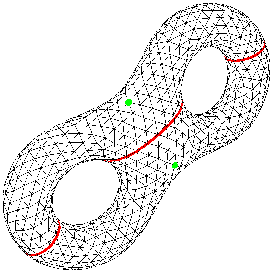
\includegraphics[width=0.45\textwidth]{figs/cvt/bisector1.png}
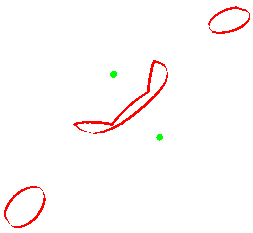
\includegraphics[width=0.45\textwidth]{figs/cvt/bisector2.png}\\
\makebox[0.9\textwidth][c]{Bisector}\\
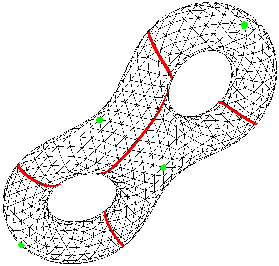
\includegraphics[width=0.45\textwidth]{figs/cvt/VD1.png}
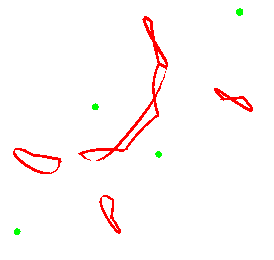
\includegraphics[width=0.45\textwidth]{figs/cvt/VD2.png}\\
\makebox[0.9\textwidth][c]{Geodesic Voronoi diagram}
\caption{Bisector and geodesic Voronoi diagram. Row 1: The bisector (red) of two sites (green) on the double-torus has three separated components. Besides line segments, a bisector on triangle mesh may also contain hyperbola segments. Row 2: The geodesic Voronoi diagram of four sites. Each Voronoi cell is bounded by two or three closed bisectors.}
\label{fig:bisector}
\end{figure}

\section{Centroidal Voronoi Tessellation }

Du et al.~\cite{Du:1999:CVT:340312.340319} first proposed the notion of the centroidal Voronoi tessellation, but long before that the similar notions
have been presented in varied areas, e.g. k-means in pattern
recognition and optimal quantization in signal processing.

The centroidal Voronoi tessellation (CVT) is a special Voronoi diagram
in which every seed $x_i$ locates at the same place with the centroid $c_i$ of its Voronoi cell $\Omega_i$ ,and was first introduced by~\cite{Du:1999:CVT:340312.340319}. But long before similar
concepts have been studied in various areas, e.g. k-means in computer vision, and pattern recognition.

To compute the CVT, one of the earliest algorithms is introduced by ~\cite{MacQueen:1967},
which is a probabilistic algorithm. Although it will surely convergence, its convergence is quite slow. Lloyd presented a deterministic
method, which is published officially in ~\cite{Lloyd:1982}. Du et al.~\cite{Du:2006:CLA:1117869.1117911} proved the convergence of Lloyd��s algorithm later.
 Because of its robustness and simplicity , Lloyd��s algorithm is
 used widely. Ju et al.~\cite{ju2002probabilistic} combined Lloyd��s algorithm with MacQueen��s method, and presented a parallel probabilistic Lloyd algorithm.
Liu et al.~\cite{Liu:2009:CVT} proved
that the energy function of CVT has $C^2$ smoothness in convex domains
and in most other commonly encountered domains with smooth density. With this $C^2$ continuity,
one can compute CVT by the quasi-Newton method (e.g. L-BFGS~\cite{liu1989limited}),
which has super linear convergence rate, thus, significantly outperforms the Lloyd
algorithm. L{\'e}vy and Liu~\cite{Levy:2010:LPC:1778765.1778856}
presented $L_p$ CVT, which generalizes CVT by minimizing a
higher-order moment of the coordinates on the Voronoi cells. This
generalization allows for aligning the axes of the Voronoi cells
with a predefined background tensor field (anisotropy). Recently,
Rong et al.~\cite{Rong:2011:CVT} extended CVT from Euclidean space
to hyperbolic and spherical space by using global parameterization.

Both the Lloyd algorithm and the Newton algorithm require computing the Voronoi
diagrams in each iteration. Although it is fairly simple to construct the
VD in Euclidean space (e.g. $\mathbb{R}^2$ and
$\mathbb{R}^3$), computing VD on curved surfaces is technically challenging.
Alliez et al.~\cite{DBLP:conf/smi/AlliezVDI03}~\cite{DBLP:journals/cvgip/AlliezVDI05} conformally parameterized genus-0 open surface
to a disk and evaluated the centroids over the density function expressed in parameter space rather than on the surface.
Thanks to the angle-preserving and local isotropic properties of conformal parameterization,
a well-shaped triangle in parameter space will not be deformed too much
once lifted back into $\mathbb{R}^3$, except for its size, which can be easily compensated by the weighted density function in $\mathbb{R}^2$.
Rong et al.~\cite{Rong:2011:CVT} generalized the CVT energy function from $\mathbb{R}^2$ to spherical space $\mathbb{S}^2$ and hyperbolic space $\mathbb{H}^2$ and then combined all of them into a unified framework - the CVT in universal covering space (UCS).
They adapted Lloyd's iteration to compute the CVT in the embedded fundamental domain of the UCS.
If a centroid is outside of the fundamental domain by one side, they performed a rigid motion to move it to the
opposite side of the fundamental domain. The adjusted centroids are
all inside the fundamental domain and are used as the new sites in the next
iteration. Rong et al.~\cite{Rong_Etc:2011} proposed a GPU-based method for computing the CVT on the plane and observed
significant speedup of these GPU-based methods over their CPU counterparts.
 Their method also works for some 3D models that can be represented as a geometry image.
However, as mentioned above, global parametrization is
computationally expensive and may suffer from serious numerical
issues if the surface has complicated geometry and non-trivial
topology. For example, the Bunny's ears are shrunk to very tiny
regions under spherical conformal
parameterization~\cite{DBLP:journals/tmi/GuWCTY04}, which poses a
great numerical challenge to compute the CVT on $\mathbb{S}^2$.

Yan et al.~\cite{DBLP:journals/cgf/YanLLSW09} proposed a different
approach. Rather than constructing the CVT on the mesh directly,
they repeatedly computed restricted Voronoi diagrams (RVD), defined
as the intersection between the input mesh and a Voronoi diagram in
$\mathbb{R}^3$. Their method uses a kd-tree to quickly identify and
compute the intersection of each triangle face with its incident
Voronoi cells. The time complexity for computing RVD is $O(m\log
n)$, where $n$ is the number of seed points and $m$ is the number of
triangles of the input mesh. Their method also adopted the
quasi-Newton method for fast convergence. They demonstrated that the
restricted RVD-based method is flexible for computing the CVT with a
non-constant density function. However, their method is embedding
space dependent and may fail on models with complicated
geometry/topology. Recently, L\'evy and
Bonneel~\cite{levy:vorpaline_imr:12} proposed an elegant method for
constructing curvature-adaptive anisotropic meshes. Their idea is to
transform the 3D anisotropic space into a higher dimensional
isotropic space, in which the mesh is optimized by computing a CVT.
L\'evy and Bonneel's method overcomes the $d$-factorial cost of
computing a Voronoi diagram of dimension $d$ by directly computing
the restricted Voronoi cells with an algorithm called Voronoi
Parallel Linear Enumeration, which can be easily parallelized. Their
method is extrinsic due to the computation of intersection between
the (higher dimensional) Voronoi cells and the surface.

\section{Discrete Geodesics}
  The discrete geodesic problem has four variations, namely,
  single-source single-destination (SSSD), single-source all-destination (SSAD), multi-source all-destination (MSAD), and all-pairs (AP).
  Among them, solving the SSAD geodesic distances and paths is of particular interest, as it is the foundation of the other three.
  Sections 2.1 and 2.2 reviews the discrete wavefront propagation methods and the PDE methods, which are two major techniques for solving the SSAD problem.
  Section 2.3 reviews the $(1+\varepsilon)$-approximation algorithms, which can guarantee the accuracy of the computed geodesic distances.
  Sections 2.4 discusses other types of discrete geodesics and the methods for computing geodesics on discrete domains other than meshes.

  \subsection{Discrete Wavefront Propagation Methods}
  \label{subsec:discretewavefront}
  Two representative methods are the MMP algorithm~\cite{Mitchell87} and the CH algorithm~\cite{Chen90},
  which simulate the wavefront propagation in a discrete manner.
  They partition mesh edges into intervals, called windows, where each window encodes the geodesic paths that are in the same face sequence.
  Then they propagate windows across mesh faces and update the geodesic distance of vertices when they are swept by some window.
  The MMP algorithm maintains a priority queue for windows and propagates the window closest to the source at a time,
  whereas the CH algorithm organizes windows in a tree and processes them in a breadth-first search order.
  Given an $n$-face mesh, the MMP algorithm runs in $O(n^2\log n)$ time and the CH algorithm has an $O(n^2)$ time complexity.
  Both algorithms have many variants, such as performance improvement~\cite{Surazhsky05},\cite{Xin09},\cite{Liu13},\cite{liu_degeneracy},\cite{fwp},
  parallelization~\cite{Ying13parallel}, and handling degeneracy~\cite{liu_degeneracy}.
  It is worth noting that there are at most $O(n^2)$ windows on an $n$-face mesh~\cite{Mitchell87},
  so the window propagation algorithms have a worst-case $O(n^2)$ time complexity on general polyhedral surfaces,
  which is known as the theoretical quadratic time barrier.
  In practice, as observed in~\cite{Surazhsky05},
  the MMP algorithm and the improved CH algorithm~\cite{Xin09} run in $O(n^{1.5}\log n)$ time on real-world meshes.

  Schreiber and Sharir~\cite{Sharir2008} proposed an elegant algorithm for computing geodesic distances on a convex polytope in $O(n\log (n))$ time,
  reaching the theoretical lower bound.
  Later, Schreiber~\cite{DBLP:journals/dcg/Schreiber10} generalized the optimal-time algorithm of convex polytope to three realistic scenarios,
  including terrain, uncrowded polyhedron and self-conforming model, which can be concave.
  These optimal-time algorithms have significant theoretical values, however, they have limited applications in computer graphics,
  since most real-world models are nonconvex.

  Kapoor~\cite{Kapoor1999} proposed an algorithm for computing shortest paths on any polyhedral surfaces in an $O(n\log^2 n)$ time complexity.
  However, due to lack of technical details, it is not possible to verify the claim.
  To date, the problem of computing \textit{exact} geodesic distances on general polyhedral surfaces in subquadratic time still remains open.

  \subsection{PDE Methods}
  \label{subsec:pde}
  The PDE methods solve the Eikonal equation $|\nabla u(x)|=1$ with boundary condition $u(s)=0$ on discrete domains, where $s$ is the source.
  In contrast to the exact methods which are computationally expensive, the PDE methods are very easy to implement and efficient.

  Using an upwind finite difference approximation to the gradient and a Dijkstra-like sweep,
  Sethian~\cite{FMM} proposed the fast marching method (FMM), which provides a solution to the Eikonal equation in time $O(n\log n)$ on a regular grid.
  A similar algorithm based on a different discretization of the Eikonal equation was developed independently by Tsitsiklis~\cite{tsit95}.
  Later, the FMM was generalized to arbitrary triangulated surfaces~\cite{FMM_ron}, unstructured meshes~\cite{Sethian2000},
  implicit surfaces~\cite{memoli2001}, parametric surfaces~\cite{spira2004} and even broken meshes~\cite{DBLP:journals/cgf/CampenK11}.
  Since the FMM uses a strict updating order and a priority queue to manage the narrow band containing the wavefront, it is non-trivial to parallelize the FMM.
  Using raster scan on a completely regular structure, Weber et al.~\cite{Weber:2008:PAA:1409625.1409626} developed a parallel FMM on geometry images,
  which runs in $O(n)$ time.
  %They implemented the algorithm on a Nvidia 8800GTX GPU and observed 4 orders of magnitude improvement in execution time.
  Other parallel methods for solving the Eiknoal equation include~\cite{zhao2007},~\cite{Fu:2011:FIM:2079141.2079157}, and~\cite{Detrixhe:2013:PFS:2442172.2442418}.

  The heat method~\cite{crane2013geodesics} is based on a completely different strategy.
  It places heat at the source vertex and then diffuses the heat in a very short time.
  Since the normalized gradient of the heat function coincides with the gradient of the geodesic distance function,
  the heat method computes the geodesic distance by solving a Poisson equation.
  %The heat method works for a wide range of discrete domains, including triangle meshes, non-planar polygonal meshes and point clouds.
  Using Cholesky factorization of the Laplacian matrix, both the heat flow and the Poisson equation can be solved at linear time.

  Recently, Belyaev and Fayolle~\cite{belyaev2015} introduced a variational approach for computing the distance to a surface (a curve in 2D)
  and proposed efficient iterative schemes for minimizing the energy functionals.
  They also investigated several PDE-based distance function approximation schemes, including Poisson distance, $p$-Laplacian distance and $L_p$-distance.

  The PDE methods work for a wide range of discrete domains, including regular grids, point clouds, and unstructured triangular and tetrahedral meshes.
  However, they provide only the first-order approximation, which is highly sensitive to mesh tessellation.

  \subsection{Other Methods}
  \label{subsec:othermethods}

  Kanai and Suzuki~\cite{Kanai2001} proposed an approximate algorithm for computing geodesic paths on polyhedral surfaces.
  The algorithm constructs a graph using the original vertices and Steiner points added on the edges.
  It computes an initial shortest path between the two given points.
  Then it iteratively improves the graph by adding more Steiner points to the region where the path passes through.
  The algorithm computes a geodesic path in $O(n\log n)$ time.
  Since the algorithm determines the location of Steiner points using heuristics, there is no theoretical guarantee of the approximation error.
  Moreover, it is not practical to extend the algorithm for the single-source geodesic distances.

  Xin et al.~\cite{DBLP:journals/tvcg/XinHF12} presented an algorithm for iteratively evolving an initial closed path on a given mesh into an exact geodesic loop.
  The algorithm has an empirical $O(mk)$ time complexity,
  where $m$ is the number of vertices in the region bounded by the initial loop and the final geodesic loop,
  and $k$ is the average number of edges in the edge sequences that the evolving loop passes through.
  Their algorithm guarantees to terminate within finite steps.

\section{Exponential Map}

With the above-mentioned discrete geodesic algorithms, we can compute the geodesic path on the surface. For any two points $p$ and $q$ on a 2-manifold surface, the geodesic
path between $p$ and $q$ is a local shortest path connecting $p$ and
$q$ on the surface \cite{doCarmo1976}. If the surface is smooth, the
geodesic is a curve on the surface whose geodesic curvature is
always zero. Since geodesic curvature is only dependent on the first
fundamental form, the geodesic is intrinsic to the surface.

 After we obtain the geodesic path, we can compute the exponential map, which defines a geodesic polar coordinate system on meshes (see Figure~\ref{fig:exp}).
Let $p\in M$ be an arbitrary point on a smooth surface $M$.
  The exponential map $\exp_p:T_pM\rightarrow M$ at $p$ is a map from the tangent plane at $p$ to $p$'s local neighborhood.
  Given a radial line on the tangent plane which originates at $p$ and has direction $\mathbf{v}\in T_pM$,
  the exponential map sends $p+t\mathbf{v}$ to a unique geodesic curve $\gamma$ originating at $p$ such that $\gamma'(0)=\mathbf{v}$ and $\|\gamma(t)\|=1$.
  Conversely, given an arc-length parameterized geodesic $\gamma$ originating at $p$, $\gamma(0)=p$, there is a unique tangent direction $\gamma'(0)$ on the tangent plane $\exp^{-1}_p(\gamma)=\gamma'(0)$. The exponential map has been used in various graphics applications, such as decal compositing~\cite{Schmidt:2006:IDC:1141911.1141930}, texture mapping~\cite{Sun:2013:TBI:2448196.2448221}, Poisson disk sampling~\cite{DBLP:journals/tvcg/YingXS013}, etc.
\begin{figure}[htbp]
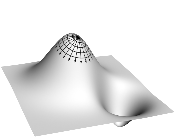
\includegraphics[width=0.45\textwidth]{figs/cvt/franke_3d.png}
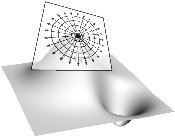
\includegraphics[width=0.45\textwidth]{figs/cvt/franke_polar.png}\\
\caption{Exponential map naturally defines a geodesic polar coordinate system on curved surfaces.}
\label{fig:exp}
\end{figure}


\section{Sampling and Shape Distribution}
  The widely used sampling techniques include blue noise~\cite{Cook:1986:SSC:7529.8927},
  point repulsion~\cite{Turk:1992:RPS:133994.134008}, centroid Voronoi tessellation (CVT)~\cite{Du:1999:CVT:340312.340319},
  stratified sampling~\cite{Nehab:2004:SPS}, spectral sampling~\cite{DBLP:journals/tog/OztireliAG10}, and polyominoes~\cite{Ostromoukhov:2007:SP:1276377.1276475}, just name a few.

  Among them, Poisson disk sampling is popular due to its nice spatial and spectral properties.
  Dart throwing~\cite{Cook:1986:SSC:7529.8927} is a popular technique to generate isotropic blue noise samples due to its simplicity.
  However, it is time consuming since a large number of trials are discarded due to conflicts.
  Many techniques have been proposed to improve the performance of dart throwing, including effective spatial data structures~\cite{Mitchell:1991:SOS:122718.122736,Dunbar:2006:SDS:1141911.1141915,Gamito:2009:AMP:1640443.1640451,Ebeida:2011:EMP:2010324.1964944},
  kernel density model~\cite{Fattal:2011:BPS:1964921.1964943}, and tile-based approaches~\cite{Cohen:2003:WTI:1201775.882265,Lagae:2005:POD:1095878.1095888,Kopf:2006:RWT:1179352.1141916,Ostromoukhov:2007:SP:1276377.1276475}.
  Wei~\cite{Wei:2008:PPD:1399504.1360619} presented the phase group algorithm
  which subdivides the sample domain into grid cells and drawing samples concurrently from multiple cells that are sufficiently far apart to avoid conflicts.
  Li~et al.~\cite{li:anisotropic:2010} generalized the isotropic blue noise sampling to the anisotropic setting.
  By using parameterization, their technique can generate high quality anisotropic sampling on surfaces.
  Bowers~et al.~\cite{Bowers:2010:PPD:1882261.1866188} extended the phase group algorithm for Poisson disk sampling on 3D surfaces.
  Wei~\cite{Wei:2010:MBN:1833351.1778816} introduced multi-class blue noise sampling where each individual class and their union exhibit blue noise properties.
  Chen et al.~\cite{Chen:2013:BBN:2508363.2508375} presented bilateral blue noise sampling for handling problems with non-spatial features.

  Bisides point based sampling, distributing 2D objects has a wide range of graphic applications.
  For example, line segment distributions are used in rendering applications, such as motion blur, defocus blur and scattering media~\cite{Sun:2013:LSS:2461912.2462023},
  and rectangle distributions are used to simulate decorative mosaics~\cite{Hausner:2001:SDM:383259.383327,battiato2013artificial}.
  Feng ~\cite{Feng:2008:ANS:1340081.1340166} generated non-overlapping ellipses with blue noise characteristic.
  Sun et al.~\cite{Sun:2013:LSS:2461912.2462023} proposed a frequency analysis of line segment sampling, which can be generalized to arbitrary non-point shapes.

  In contrast to the 2D counterpart, shape distribution on 3D surfaces remains largely unexplored.
  Bowers et al.~\cite{Bowers:2010:PPD:1882261.1866188} computed Poisson disk distributions on 3D surfaces by space partition.
  With a global parameterization, Li et al.~\cite{li:anisotropic:2010} presented an algorithm to distribute ellipse samples that exhibit anisotropic blue noise properties on 3D surfaces.
  They also evaluated the spectrum of anisotropic blue noise by warping and sphere sampling.
